% Compact PGFPlots panel for sampled surface11 BSC bit-scale decomposition.
% Requires \usepackage{pgfplots} and \pgfplotsset{compat=1.18}.
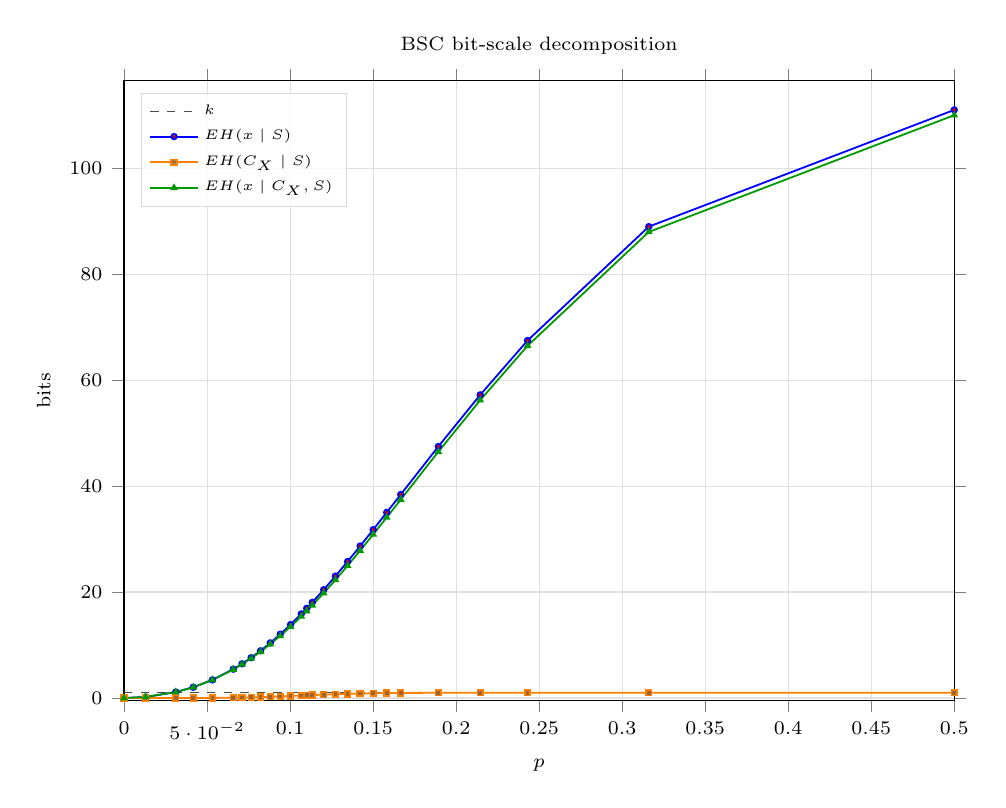
\begin{tikzpicture}
\begin{axis}[
  name=Surface11BSCBitScaleAxis,
  width=\linewidth,
  height=0.78\linewidth,
  title={BSC bit-scale decomposition},
  title style={font=\scriptsize},
  xlabel={$p$},
  ylabel={bits},
  xmin=0, xmax=0.5,
  ymin=-0.5, ymax=116.55,
  grid=both,
  major grid style={black!12},
  minor grid style={black!6},
  tick align=outside,
  tick label style={font=\scriptsize},
  label style={font=\scriptsize},
  legend cell align={left},
  legend style={draw=black!15, fill=white, fill opacity=0.82, text opacity=1, at={(0.02,0.98)}, anchor=north west, font=\tiny},
]
\addplot[black!70, dashed, line width=0.55pt] coordinates {(0,1) (0.5,1)};
\addlegendentry{$k$}
\addplot+[color=blue, mark=*, mark size=1.0pt, line width=0.65pt]
coordinates {(0,0) (0.0129868620555,0.190087251929) (0.0311244603048,1.1236084421) (0.0416926902737,2.03112781761) (0.0532390407768,3.4208840072) (0.0657867063546,5.44393749382) (0.0710958755299,6.46410425371) (0.0765765344037,7.61082287369) (0.0822333323659,8.91790354787) (0.0880715694979,10.4051368886) (0.0940972433461,12.0473432476) (0.100317108961,13.8552006774) (0.106738753821,15.8609212097) (0.110027864438,16.9297343805) (0.113370689941,18.0500912287) (0.120222466333,20.4308249167) (0.127304805976,23.003936446) (0.134629772869,25.7533472518) (0.142210976498,28.6823502277) (0.150063823499,31.76788143) (0.158205829694,35.0209108588) (0.166657010397,38.4142965608) (0.189297705371,47.4714153738) (0.21450174486,57.213821505) (0.243003853809,67.4689364889) (0.316019346324,88.9615858148) (0.5,111)};
\addlegendentry{$\mathbb{E}H(x\mid S)$}
\addplot+[color=orange, mark=square*, mark size=1.0pt, line width=0.65pt]
coordinates {(0,0) (0.0129868620555,2.12815097741e-08) (0.0311244603048,0.000274528336446) (0.0416926902737,0.0041281086682) (0.0532390407768,0.0188533128908) (0.0657867063546,0.0591293290166) (0.0710958755299,0.0871471837581) (0.0765765344037,0.1242544701) (0.0822333323659,0.173499810097) (0.0880715694979,0.234245262654) (0.0940972433461,0.30683506349) (0.100317108961,0.383750167317) (0.106738753821,0.468570924082) (0.110027864438,0.510522171227) (0.113370689941,0.552181796508) (0.120222466333,0.635811471181) (0.127304805976,0.713658008454) (0.134629772869,0.782982954551) (0.142210976498,0.842301655738) (0.150063823499,0.889510289958) (0.158205829694,0.927980727232) (0.166657010397,0.95528991618) (0.189297705371,0.989561956385) (0.21450174486,0.998626670396) (0.243003853809,0.999928648004) (0.316019346324,1.0000005697) (0.5,1)};
\addlegendentry{$\mathbb{E}H(C_X\mid S)$}
\addplot+[color=green!60!black, mark=triangle*, mark size=1.0pt, line width=0.65pt]
coordinates {(0,0) (0.0129868620555,0.190087230647) (0.0311244603048,1.12333391376) (0.0416926902737,2.02699970894) (0.0532390407768,3.4020306943) (0.0657867063546,5.3848081648) (0.0710958755299,6.37695706996) (0.0765765344037,7.48656840359) (0.0822333323659,8.74440373778) (0.0880715694979,10.1708916259) (0.0940972433461,11.7405081841) (0.100317108961,13.4714505101) (0.106738753821,15.3923502856) (0.110027864438,16.4192122093) (0.113370689941,17.4979094322) (0.120222466333,19.7950134455) (0.127304805976,22.2902784375) (0.134629772869,24.9703642972) (0.142210976498,27.8400485719) (0.150063823499,30.8783711401) (0.158205829694,34.0929301316) (0.166657010397,37.4590066446) (0.189297705371,46.4818534175) (0.21450174486,56.2151948346) (0.243003853809,66.4690078409) (0.316019346324,87.9615852451) (0.5,110)};
\addlegendentry{$\mathbb{E}H(x\mid C_X,S)$}
\end{axis}
\end{tikzpicture}
